% -- %% ============================ Tufte' handout ===============================
% -- \documentclass[nobib]{tufte-handout}
% -- 
% -- %% ------------------------------ Tables -------------------------------------
% -- \usepackage{blkarray}          % convenient matrices
% -- \usepackage{rotating}          % rotate objects
% -- \usepackage{booktabs}          % book-quality tables
% -- \usepackage{units}             % non-stacked fractions and better unit spacing
% -- \usepackage{multicol}          % multiple column layout facilities
% -- \usepackage{lipsum}            % filler text
% -- \usepackage{fancyvrb}          % extended verbatim environments
% -- \fvset{fontsize=\normalsize} % font size for fancy-verbatim environments
% -- \usepackage{tabularx,ragged2e} % table formatting
% -- \usepackage{array}             % table formatting
% -- \usepackage{siunitx}           % alignment
% -- \sisetup{detect-all}
% -- \sisetup{input-symbols = ()}
% -- \usepackage{adjustbox}         % scaling
% -- \usepackage[T1]{fontenc}       % text
% -- \newcolumntype{P}[1]{>{\centering\arraybackslash}p{#1}}
% -- \usepackage{xcolor}            % coloured text etc.% 
% -- 
% -- %% --------- Standardize command font styles and environments ----------------
% -- \newcommand{\doccmd}[1]{\texttt{\textbackslash#1}}% adds backslash
% -- \newcommand{\docopt}[1]{\ensuremath{\langle}\textrm{\textit{#1}}\ensuremath{\rangle}}% optional command argument
% -- \newcommand{\docarg}[1]{\textrm{\textit{#1}}}% (required) command argument
% -- \newcommand{\docenv}[1]{\textsf{#1}}% environment name
% -- \newcommand{\docpkg}[1]{\texttt{#1}}% package name
% -- \newcommand{\doccls}[1]{\texttt{#1}}% document class name
% -- \newcommand{\docclsopt}[1]{\texttt{#1}}% document class option name
% -- \newenvironment{docspec}{\begin{quote}\noindent}{\end{quote}}% command specification environment
% -- 
% -- %% ----------------------------- Links ---------------------------------------
% -- \hypersetup{
% --     colorlinks=true,
% --     linkcolor=RoyalBlue,
% --     filecolor=RoyalBlue,      
% --     urlcolor=RoyalBlue,
% --     citecolor=Black,
% --     pdftitle={Overleaf Example},
% --     pdfpagemode=FullScreen,
% --     }
% --   
% -- %% -------------------------- Drawing and plots ------------------------------
% -- \usepackage{pgfplots}
% -- \pgfplotsset{compat=1.16}              % pgf plots
% -- \usepackage{pgf}
% -- \usepackage[utf8]{inputenc}\DeclareUnicodeCharacter{2212}{-}
% -- \usepackage{tikz}                      % tikz plots
% -- \usetikzlibrary{positioning}
% -- \usetikzlibrary{arrows.meta}
% -- \usetikzlibrary{backgrounds}
% -- \usetikzlibrary{calc}
% -- \usetikzlibrary{matrix}
% -- \usetikzlibrary{decorations.pathreplacing}
% -- \usetikzlibrary{fit}
% -- \def\firstcircle{(0,0) circle (1.5cm)} % custom shapes
% -- \def\secondcircle{(0:2cm) circle (1.5cm)}
% -- \colorlet{circle edge}{black!50}
% -- \colorlet{circle area}{black!20}
% -- \tikzset{filled/.style={fill=circle area, draw=circle edge, thick},
% -- outline/.style={draw=circle edge, thick}}
% -- \usepackage{tikz-network}
% -- \usepackage{sparklines}
% --   
% -- %% ----------------------------- Options -----------------------------------
% -- \usepackage{geometry}
% -- \renewcommand{\baselinestretch}{0.85}
% -- \usepackage{graphicx}          % allow embedded images
% --   \setkeys{Gin}{width=\linewidth, totalheight=\textheight, keepaspectratio}
% --   \graphicspath{{graphics/}}
% -- \usepackage{amsmath}                  % extended mathematics
% -- \usepackage[scaled=0.9]{helvet}       % sans-serif font to use
% -- \usepackage[defaultmathsize, symbolgreek]{mathastext}
% -- %\renewcommand\familydefault\sfdefault
% -- \Mathastext[helvet]
% -- \usepackage{sansmath}                 % maths with sans-serif
% -- \AtBeginEnvironment{tikzpicture}{\sansmath}
% -- \AtEndEnvironment{tikzpicture}{\unsansmath}
% -- \setsidenotefont{\sffamily\small}
% -- \setcaptionfont{\sffamily\small}
% -- \setmarginnotefont{\sffamily\small}
% -- \setcitationfont{\sffamily\small}
% -- 
% -- %% ----------------------------- Quotations ----------------------------------
% -- \usepackage{dirtytalk}
% -- 
% -- %% ------------------------------- Authors -----------------------------------
% -- \usepackage{authblk}
% -- 
% -- %% ----------------------------- References ----------------------------------
% -- %\usepackage[colorlinks, citecolor=DarkOrange]{hyperref}
% -- \usepackage[
% --   style=verbose,
% --   autocite=footnote,
% --   backend=biber,
% --   citestyle=authoryear
% -- ]{biblatex}
% -- \addbibresource{references/main_biblio.bib}
% -- \addbibresource{references/appendix_biblio.bib}

%% ============================ Classic wp ===================================
\documentclass[11pt]{article}

% ------------------------- Page and paragraph layout ------------------------
\usepackage[a4paper]{geometry}
\geometry{verbose,tmargin=1in,bmargin=1in,lmargin=1in,rmargin=1in}
%\setcounter{secnumdepth}{-2}
%\setcounter{tocdepth}{-2}
\usepackage{setspace}
\onehalfspacing%\doublespacing
\setlength{\parindent}{2.75em}
\setlength{\parskip}{1em}
%\renewcommand{\baselinestretch}{1.5}
\usepackage{titlesec}
\titlespacing{\section}{0pt}{1.5ex}{-1.5ex}
\titlespacing{\subsection}{0pt}{1.5ex}{-1.5ex}
\titlespacing{\subsubsection}{0pt}{1.5ex}{-1.5ex}
%\makeatletter
%\renewcommand{\@seccntformat}[1]{}
%\makeatother

%% -------------------------- Info on authors --------------------------------
\usepackage{authblk}

%% --------------------------- Text style ------------------------------------
\usepackage{color}

%% ----------------------------- Endnote -------------------------------------
%\usepackage{endnotes}
%\let\footnote=\endnote

%% ------------------------------- Links ------------------------------------- 
\usepackage[dvipsnames]{xcolor}
\usepackage[
	colorlinks=true,
	allcolors=base_c,
	%citecolor=CadetBlue,
	%urlcolor=CadetBlue
	]{hyperref}%
 
%% --------------------------- Bibliography ----------------------------------
\usepackage[
%natbib=true,
backend=biber,
style=alphabetic,
citestyle=authoryear,
%citestyle=apa,
%hyperref=true,
%maxbibnames=99,
%firstinits=false
maxcitenames=4,
%citetracker=true,
%parentracker=true,
bibstyle=authortitle
]{biblatex}

%% --------------------------- Exhibits --------------------------------------
\usepackage{array}
\usepackage{booktabs}
\usepackage{dcolumn}
\usepackage{pgf}
\usepackage{lmodern}
\usepackage{import}
\usepackage{pgfplots}
\pgfplotsset{compat=1.16}
\usepackage[utf8]{inputenc}\DeclareUnicodeCharacter{2212}{-}
\usepackage{tikz}
%\usepackage{tabularx,ragged2e}
\usepackage{threeparttable}
\usepackage{graphicx}
\usepackage{rotating}
%\usepackage[T1]{fontenc}
%\usepackage{times}
%\usepackage{amsmath}
%\usepackage{mathptmx}
%\usepackage{bbm}
%\usepackage{dsfont}
%\usepackage{etoolbox}
\usepackage{caption}
\captionsetup[table]{labelfont=sc, labelsep=newline}
\renewcommand{\figurename}{Fig.}
%\usepackage{ctable}
\renewcommand{\thetable}{\Roman{table}}
\usepackage{csquotes}

% -------------------------- Special chars -----------------------------------
\usepackage{amssymb}

% --------------------------- Appendices -------------------------------------
\usepackage[toc, page]{appendix}

% -------------------------- Tikz charts -------------------------------------
\definecolor{base_c}{HTML}{6A94D5}
\definecolor{comp_c}{HTML}{D5AB6A}
\definecolor{tri_1_c}{HTML}{D56A94}
\definecolor{tri_2_c}{HTML}{94D56A}
\definecolor{tet_1_c}{HTML}{D56ACA}
\definecolor{tet_2_c}{HTML}{D5AB6A}
\definecolor{tet_3_c}{HTML}{6AD575}

% =============================== References =================================
% ------------------------------ Load biblio ---------------------------------
\addbibresource{references/main_biblio.bib}
\addbibresource{references/appendix_biblio.bib}

%% =============================== Document ==================================
%% ------------------------------ Cover page ---------------------------------
%% Title
\title{Exogenous Shocks in Leadership and Management Research:\\
Types, Challenges, and Opportunities\vspace{2em}}

%% Author
\author[$\bullet$]{Simone Santoni}
\author[$\star$]{Jost Sieweke}
\author[$\circ$]{Michael Withers}
\affil[$\bullet$]{Bayes Business School --- City, University of London}
\affil[$\star$]{Vrije Universiteit Amsterdam}
\affil[$\circ$]{Mays Business School --- Texas A\&M University}

\renewcommand\Authands{and}
%\renewcommand\Authfont{\sffamily}
\renewcommand\Affilfont{\normalsize}

%% Date
\date{\vspace{1em} \normalsize \today \vspace{1em} \\ 
      \textcolor{red}{(Structured draft --- do not circulate)}}

%% ---------------------------- Body of the document -------------------------
\begin{document}

\begin{singlespace}

\maketitle

\begin{abstract}

---Abstract goes here---

\bigskip

\textit{Keywords}: kw1, kw2, kw3.

\end{abstract}

\end{singlespace}

\clearpage

\begin{refsection}[references/main_biblio.bib]

\section{Introduction}
\label{sec:introduction}

%% recall causal inference issues, mention attempts made by the community
% to improve causal inference, and connect these efforts with the popularity
% of natural experiments

The quest for empirical identification in management research has created
substantial attention around `natural experiments,' a form of causal inquiry
that has been traditionally popular in economics
\parencite[][]{Meyer1995,Rosenzweig2000} and political science
\parencite[][]{Dunning2008}.  The premise to conduct a natural experiment is the
presence of a `naturally' occurring event --- such as new regulations and laws,
natural disasters, or economic and political crises --- that heterogeneously
influences the units of a population \parencite[][]{Dunning2012,Robinson2009}.
Insofar as such event generates random or as-if random variations in the
environment, scholars can mimic the experimental ideal in which units are split
into a treatment and a control group or receive different levels of the
treatment. Ultimately, this opens up the possibility of inferring causal effects
when the substantive relationship at hand is difficult to investigate in a
laboratory setting and/or require operating costly, impractical, or unethical
field experiments.

% motivation for the article - NEs are not rooted in the field of strategic
% mangagement; rather, they are emerging as one of the most popular ways to
% tackle on the endogeneity challenge. As NEs diffuse in management research,
% pracrices emerge and crystallize on how to discover and leverage exogenous
% variations in order to test causal relationships. 

Although naturally occurring events can turn into opportunities to conduct
causal research, there are limited guidelines that help management scholars
prepare and review papers that implement the natural experiment research design.
To fill this gap, we highlight the strengths and weaknesses of natural
experiments as operated in the field of management studies and propose
actionable suggestions to assess and communicate the validity of natural
experiments.

To do so, we critically review the population of 147 natural experiments
published across seventeen top-tier management journals.\footnote{\todo{We're
updating the literature search on May 31, 2021.}} Our review aims
to address the following research questions: \emph{R1 --- How do management
scholars claim the random or as-if random nature of environmental variation at
the core of a natural experiment? R2 --- How do they claim the empirical and
substantive relevance of a natural experiment? R3 --- How do they claim the
credibility of the statistical model encapsulated in a natural experiment
design?}

% what we do - we survey papers adopting a NE research design and take stock of
% the emerging practices. Then, we analyze these practices through a validity
% framework (i.e., Dunning's framework) in order to highlight critical
% areas/dimensions along which NE applications can be improved. Finally, we
% provide guidelines that help reviewers and authors in analyzing the validity
% of a NE paper

% contribution of the article - we aim at assisting scholars to get the most out
% of the NE paper and clarify the expectations about what a 'good' quality NE
% paper is (this could smooth the review process)


% organization of the article
This work is organized as follows. The next two sections briefly introduce the
key features of the `standard natural experiment,' \footnote{In his
comprehensive, cross-disciplinary analysis of the literature, Dunning
\citeyear[][]{Dunning2012} identifies three forms of natural experiments:
Standard natural experiments; instrumental variables (Angrist, 1990); regression
discontinuity designs (Thistlethwaite \& Campbell, 1960). In the interest of
clarity and integrity, our review concentrates on standard natural experiments,
whose origin goes back to the highly acclaimed and impactful research Dr John
Snow (Snow, 1855) conducted on the diffusion of cholera in the mid
19\textsuperscript{th} century London. In this paper we use the term `natural
experiment' to exclusively refer to standard natural experiments.} along with
the evaluative framework we use to analyze the individual natural experiments.
The following section describes the selection of the reviewed studies. Then, we
present the key insights that emerge from our analysis and conclude with a
suggested checklist that helps management scholars to exploit the opportunities
of causal inference offered by naturally occurring events. The online appendix
presents an integrated set of Python scripts to implement standard natural
experiments and to assess their validity.\footnote{\todo{Jost and I have been
working on a Python library that provides an integrated set of statistical and
visualization capabilities for the analysis of natural experiments. Happy to
share what we have produced so far.}}


.

\section{What is an exogenous shock?}
\label{sec:what_exogenous_shocks}

\subsection{Exogenous shocks in the literature on natural experiments}
\label{subsec:exogenous_shocks_and_ne}




\begin{figure}[!htbp]
  %\sffamily
  \centering
  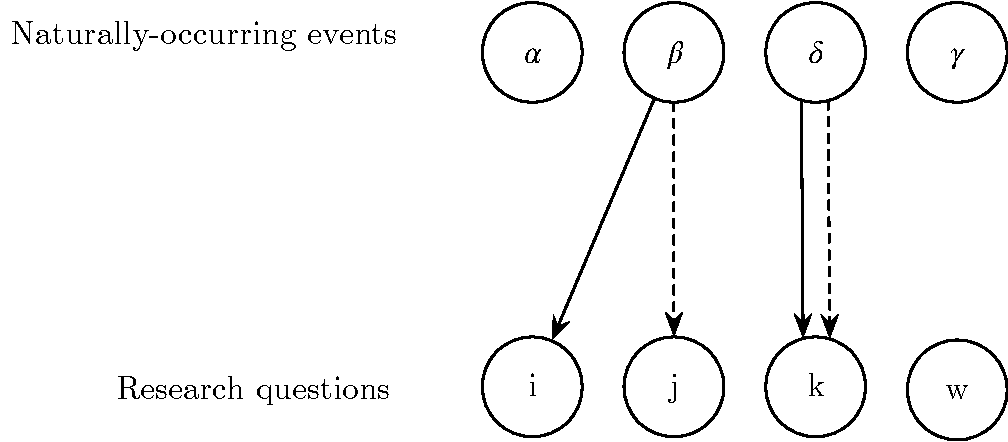
\includegraphics[width=0.7\textwidth]{exhibits/event_rq_mapping.pdf}
  \caption{Exogenous shocks map naturally-occurring events onto 
  research questions via empirical and substantive relevance. Notes:
  
\includegraphics[width=0.075\textwidth]{exhibits/event_rq_mapping_0.pdf}
  = empirical relevance; 
  
\includegraphics[width=0.075\textwidth]{exhibits/event_rq_mapping_1.pdf}
   = substantive relevance.}
  \label{fig:event_rq_mapping}
\end{figure}



\begin{figure}[!htbp]
  %\sffamily
  \centering
  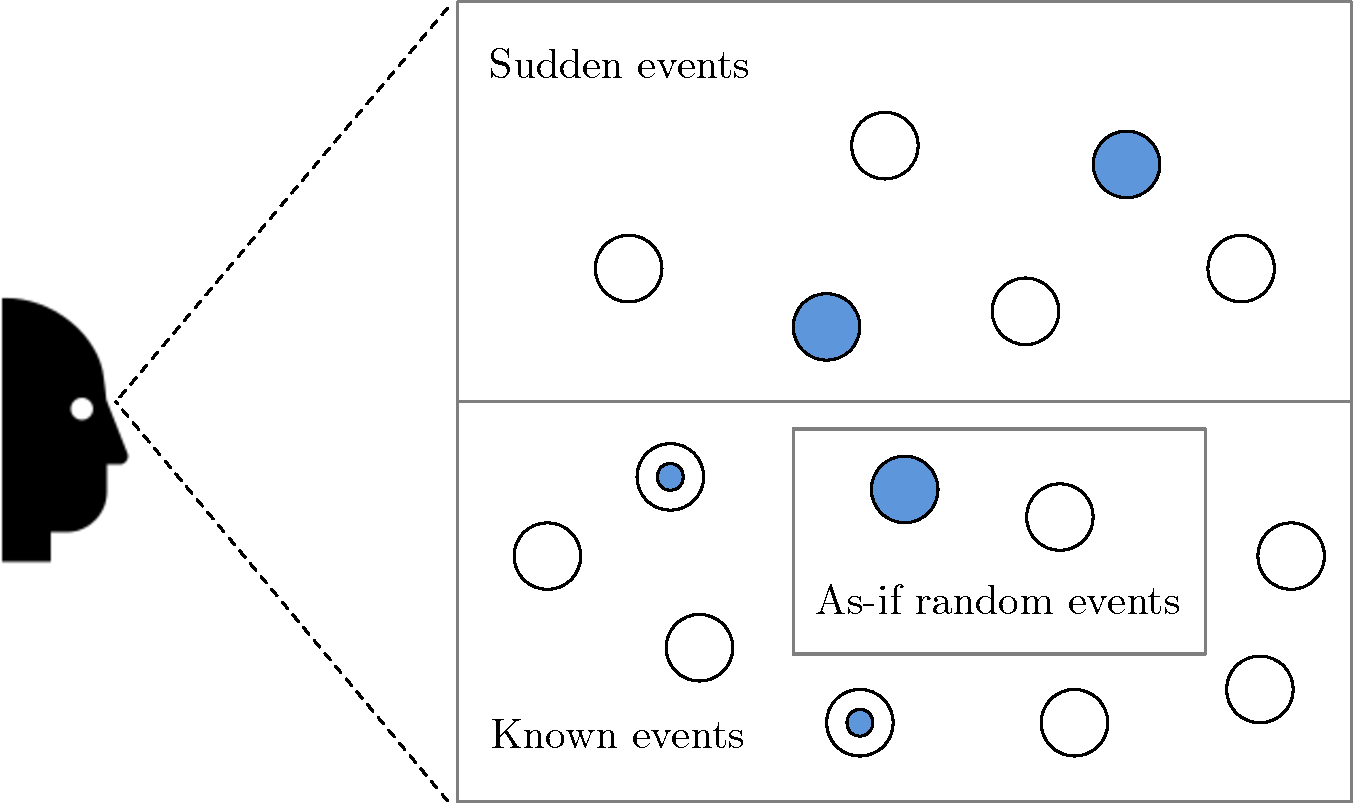
\includegraphics[width=0.75\textwidth]{exhibits/exogenous_shocks_and_ne.pdf}
  \caption{Semantic representation of exogenous shocks in the natural 
  experiment literature. Notes:  
  
\includegraphics[width=0.0175\textwidth]{exhibits/exogenous_shocks_and_ne_0.pdf}
  = exogenous shocks;
  
\includegraphics[width=0.0175\textwidth]{exhibits/exogenous_shocks_and_ne_1.pdf}
  = events that have substantive relevance but do not support causal inference;
  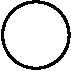
\includegraphics[width=0.0175\textwidth]{exhibits/exogenous_shocks_and_ne_2.pdf}
  = events that lack empirical and substantive relevance.}
  \label{fig:exogeneous_shocks_and_ne}
\end{figure}

\subsection{Exogenous shocks in leadership and management research}
\label{subsec:exogenous_shocks_in_management}

\noindent The literature on natural experiments offers meaningful elements 
to clarify the nature and potential impact of exogenous shocks (\cite[for an 
overview of the natural experiment design, see for example][]{withers_li_2021,
dunning_2012,craig_et_al_2017};\cite{sieweke_santoni_2020}). 

\begin{figure}[!htbp]
    \centering
    \import{}{exhibits/studies_over_time.pgf}
    \caption{Distribution of studies that claim to use an exogenous shock across
    management journals.  Notes: N = 32; in the interest of consistency, we
    excluded `exogenous shock' studies published in Management Science addressing
    finance or operations problems. The following journals do not have any
    `exogenous shock' study: Administrative Science Quarterly, Entrepreneurship
    Theory and Practice, Journal of Business Venturing, Journal of Management,
    Leadership Quarterly, Research Policy.}
    \label{fig:studies_across_journals}
\end{figure}         



\begin{figure}[!htbp]
    \centering
    \import{}{exhibits/classes_of_events.pgf}
    \caption{Classes of naturally-occurring events presumed to create exogenous shocks.}
    \label{fig:classes_of_events}
\end{figure}



\begin{figure}[!htbp]
    \centering
    \import{}{exhibits/event_roles.pgf}
    \caption{Role of the naturally-occurring events presumed to create exogenous shocks.}
    \label{fig:event_roles}
\end{figure}



\clearpage

% define new column type
\newcolumntype{Y}[1]{%
  >{\small\raggedright\everypar{\hangindent=1em}\arraybackslash}p{#1}%
}
% define newline to use hangindent on new line
\renewcommand{\arraystretch}{1.3}

\begin{sidewaystable}[!htbp]
  \centering
  %\sffamily
  \begin{small}
    \caption{Summary of study events, research questions, and exogenous shocks}
    \vspace{-1.75em}
    \label{tab:}
    \begin{center}
       %\resizebox{1\textwidth}{!}{%
       \begin{tabular}{{@{\extracolsep{2pt}} 
         p{3.85cm}@{\hskip 4mm}   %1 
         Y{4cm}@{\hskip 4mm}   %2
         Y{4cm}@{\hskip 4mm}   %3
         p{0.5cm}@{\hskip 4mm}   %4
         p{0.5cm}@{\hskip 4mm}   %5
         Y{7cm}@{\hskip 4mm} %6
         }}
         \toprule \toprule
         & %1
         & %2
         & %3
         \multicolumn{3}{l}{Relevance of the event}\\ \cmidrule{4-6}
         \multicolumn{1}{l}{Study} &
         \multicolumn{1}{l}{Event} &
         \multicolumn{1}{l}{Research question} &
         \multicolumn{1}{c}{Empirical} &
         \multicolumn{1}{c}{Substantive} &
         \multicolumn{1}{l}{Summary}\\
         \midrule \\[-1.8ex]

         Birhanu \& Wezel \parencite*{gedefawbirhanu2020}\dotfill &
         Government changes following Arab spring social movement. &
         How does group affiliation influence firm performance under weak market
         institutions?&
         \multicolumn{1}{c}{$\checkmark$} &
         \multicolumn{1}{c}{$\times$} &
         The use of sudden government change is presumed to affect executives'
         capacity to influence political leaders.\\ \\[-1.8ex]

         Byun et al. \parencite*{byun20191368}\dotfill&
         Change in a politician's committee and/or committee chair assignments. &
         How do changes in an employee's relational capital influence mobility 
         and entrepreneurship decisions? &
         \multicolumn{1}{c}{$\times$} &
         \multicolumn{1}{c}{$\checkmark$} &
         Lobbyists may experience a discontinuous shift in the value associated
         with a connection if there are changes to a politician's committee
         and/or committee chair assignments. Then, the authors can
         investigate empirically the consequences of social capital change on
         lobbyists' career. \\ \\[-1.8ex]
         
         Cabral et al. \parencite*{cabral202128}\dotfill&
         Staggered passage of anti-takeover laws in U.S. &
         Does managerial job security affect the adoption of innovative 
         practices and structures?&
         \multicolumn{1}{c}{$\checkmark$} &
         \multicolumn{1}{c}{$\checkmark$} &
         The adoption of an anti-takeover statute is a proxy of managerial job
         security, which changes across states and within individual states over
         time, and is supposed to affect the propensity to create a CVC
         program. \\ \\[-1.8ex]

         Cai \& Shi \parencite*{cai2019159}\dotfill &
         Revelation of the sex abuse of children by Catholic priests in U.S. &
         Does a firm's religious environment influence outside parties' 
         perceptions in contracting with the firm? &
         \multicolumn{1}{c}{$\checkmark$} &
         \multicolumn{1}{c}{$\times$} &
         Revelation of the sex abuse of children by Catholic priests is an
         exogenous shock to the religiosity of a region, which  can 
         influence the capital structure, credit rating, cost of debt, and
         covenants of local firms.\\ \\[-1.8ex]
         \bottomrule
       
        \end{tabular}
       %} 
    \end{center}
  \end{small}
\end{sidewaystable}

\begin{sidewaystable}[!htbp]
  \centering
  %\sffamily
  \begin{small}
    \caption*{\textsc{Table I} (cont'd)}
    \vspace{-1.75em}
    \label{tab:}
    \begin{center}
       %\resizebox{1\textwidth}{!}{%
       \begin{tabular}{{@{\extracolsep{2pt}}
         p{4.20cm}@{\hskip 4mm}   %1 
         Y{4cm}@{\hskip 4mm}   %2
         Y{4cm}@{\hskip 4mm}   %3
         p{0.5cm}@{\hskip 4mm}   %4
         p{0.5cm}@{\hskip 4mm}   %5
         Y{7cm}@{\hskip 4mm} %6
         }}
         \toprule \toprule
         & %1
         & %2
         & %3
         \multicolumn{3}{l}{Relevance of the event}\\ \cmidrule{4-6}
         \multicolumn{1}{l}{Study} &
         \multicolumn{1}{l}{Event} &
         \multicolumn{1}{l}{Research question} &
         \multicolumn{1}{c}{Empirical} &
         \multicolumn{1}{c}{Substantive} &
         \multicolumn{1}{l}{Summary}\\
         \midrule \\[-1.8ex]

         Chatterji \& Fabrizio \parencite*{chatterji2016447}\dotfill&
         Department of Justice investigation against the five largest U.S. 
         orthopedic device makers.&
         How does an open system of innovation affect the rate and direction 
         of innovation?&
         \multicolumn{1}{c}{$\checkmark$} &
         \multicolumn{1}{c}{$\times$} &       
         Department of Justice investigation increases the frictions in the 
         market for ideas, by regulating the interactions between physicians 
         and the medical device firms under investigation.\\
         \\[-1.8ex]
         
         Chatterji \& Toffel \parencite*{chatterji2010917}\dotfill&
         Change in the scope of KLD Database, a prominent source of CSR ratings.&
         How do managers react to poor corporate environmental ratings?&
         \multicolumn{1}{c}{$\checkmark$} &
         \multicolumn{1}{c}{$\checkmark$} &       
         The change in KLD's scope creates a subset of
         companies responding for the first time to a CSR rating, which allows
         the authors to deal with mutual causality issues regarding a firm's CSR
         rating and CSR strategy.\\ \\[-1.8ex]
         
         Chen \& Garg \parencite*{chen20181239}\dotfill &
         Injuries occurring to star NBA players. &
         Does a star's temporary absence help the organization overcome myopia?&
         \multicolumn{1}{c}{$\times$} &
         \multicolumn{1}{c}{$\checkmark$} &       
         The absence of star players is presumed to impact the pattern of
         organizational routines at the team level. \\ \\[-1.8ex]
         
         Choudhury \& Kim \parencite*{choudhury2019203}\dotfill&
         Change in U.S. H1B employment visas.&
         How do migrant inventors influence knowledge production and reuse? &
         \multicolumn{1}{c}{$\times$} &
         \multicolumn{1}{c}{$\checkmark$} &
         The H1B quota change exempted universities and a selected list of other
         entities, creating heterogeneous effects in terms of supply of first-generation
         ethnic migrant inventors and the rate of codification of knowledge
         previously locked within migrant inventors' home countries.\\ \\[-1.8ex]

         \bottomrule
        \end{tabular}
        %} 
      \end{center}
    \end{small}
  \end{sidewaystable}
  
\begin{sidewaystable}[!htbp]
    \centering
    %\sffamily
    \begin{small}
      \caption*{\textsc{Table I} (cont'd)}
      \vspace{-1.75em}
      \label{tab:}
      \begin{center}
        %\resizebox{1\textwidth}{!}{%
        \begin{tabular}{{@{\extracolsep{2pt}}
          p{3.85cm}@{\hskip 4mm}   %1 
          Y{4cm}@{\hskip 4mm}   %2
          Y{4cm}@{\hskip 4mm}   %3
          p{0.5cm}@{\hskip 4mm}   %4
          p{0.5cm}@{\hskip 4mm}   %5
          Y{7cm}@{\hskip 4mm} %6
          }}
          \toprule \toprule
          & %1
          & %2
          & %3
          \multicolumn{3}{l}{Relevance of the event}\\ \cmidrule{4-6}
          \multicolumn{1}{l}{Study} &
          \multicolumn{1}{l}{Event} &
          \multicolumn{1}{l}{Research question} &
          \multicolumn{1}{c}{Empirical} &
          \multicolumn{1}{c}{Substantive} &
          \multicolumn{1}{l}{Summary}\\
          \midrule \\[-1.8ex]

         Chown \& Liu \parencite*{chown2015177}\dotfill &
         Turnover within U.S. Senate and `iconoclastic' senators deviating from 
         the institutionalized seating arrangement. &
         How does one's location in an organizational forum affect the
         likelihood to receive support from peers?&
         \multicolumn{1}{c}{$\checkmark$} &
         \multicolumn{1}{c}{$\times$} &
         Turnover within U.S. Senate and `iconoclastic' senior senators create
         opportunities for freshman senators not to seat at the margins of the
         chamber. These elements affect the dyadic distance between senators, a factor
         that is presumed to affect the likelihood of joint support. \\ \\[-1.8ex]

         Corbo et al. \parencite*{corbo2016323}\dotfill&
         9/11.&
         Does a major environmental shock affect the social structure of an 
         organizational field?&
         \multicolumn{1}{c}{$\times$} &
         \multicolumn{1}{c}{$\checkmark$} &
         9/11 is supposed to affect the organization and functioning of civil
         aviation, which allows the authors to assess the extent with which
         network mechanisms shape the alliances connecting airline companies 
         under different contingencies.\\ \\[-1.8ex]

         Drexler \& Schoar \parencite*{drexler20142722}\dotfill &
         Sick leave episodes among loan officers &
         How (much) does employee turnover affect organizational performance? &
         \multicolumn{1}{c}{$\checkmark$} &
         \multicolumn{1}{c}{$\checkmark$} &
         Loan officers' sick leaves alter economic and social exchange between
         the firm and its clients.\\ \\[-1.8ex]
        
         Gupta et al. \parencite*{gupta2020802}\dotfill &
         Sarbanes-Oxley Act (SOX) \& Global Financial Crisis &
         Does CFO gender influence the likelihood of financial misreporting? &
         \multicolumn{1}{c}{$\checkmark$} &
         \multicolumn{1}{c}{$\times$} &
         The authors expect: i) SOX to lead to a larger decrease in financial
         misreporting for male CFO firms than female-CFO firm; ii) firms to face
         greater pressure to report favorable earnings during crisis periods,
         which is more likely to influence male compared to female CFOs (based
         on the logic that female CFOs will be less likely to engage in fraud
         regardless of stakeholder pressure).\\  \\[-1.8ex]
          
         \bottomrule
       \end{tabular}
       %} 
    \end{center}
  \end{small}
\end{sidewaystable}

\begin{sidewaystable}[!htbp]
  \centering
  %\sffamily
  \begin{small}
    \caption*{\textsc{Table I} (cont'd)}
    \vspace{-1.75em}
    \label{tab:}
    \begin{center}
       %\resizebox{1\textwidth}{!}{%
       \begin{tabular}{{@{\extracolsep{2pt}}
         p{3.85cm}@{\hskip 4mm}   %1 
         Y{4cm}@{\hskip 4mm}   %2
         Y{4cm}@{\hskip 4mm}   %3
         p{0.5cm}@{\hskip 4mm}   %4
         p{0.5cm}@{\hskip 4mm}   %5
         Y{7cm}@{\hskip 4mm} %6
         }}
         \toprule \toprule
         & %1
         & %2
         & %3
         \multicolumn{3}{l}{Relevance of the event}\\ \cmidrule{4-6}
         \multicolumn{1}{l}{Study} &
         \multicolumn{1}{l}{Event} &
         \multicolumn{1}{l}{Research question} &
         \multicolumn{1}{c}{Empirical} &
         \multicolumn{1}{c}{Substantive} &
         \multicolumn{1}{l}{Summary}\\
         \midrule \\[-1.8ex]

         Haveman et al. \parencite*{byun20191368}\dotfill&
         California Legislature enactment of the nation's first comprehensive 
         managed competition program, and Garn-St. Germain Act&
         How do organizations respond to discontinuous indsutry-level change?&
         \multicolumn{1}{c}{$\times$} & 
         \multicolumn{1}{c}{$\checkmark$} &
         The authors use a series of regulatory changes to investigate how
         organizations respond to punctuated changes in the environment and with
         what performance consequences.\\ \\[-1.8ex]
          
         Hilary \& Huang \parencite*{hilary2021}\dotfill &
         Revelation of the sex abuse of children by Catholic priests in U.S. &
         Does generalized trust affect the power of CEO contracts? & 
         \multicolumn{1}{c}{$\checkmark$} & 
         \multicolumn{1}{c}{$\times$} &
         Revelation of the sex abuse of children by Catholic priests
         reduces generalized trust for certain counties only, which helps to reveal
         the causal effect of generalized trust on the characteristics of
         executives' contracts.\\ \\[1.8ex] 

         Jie et al. \parencite*{jia2020290}\dotfill&
         2005 Regulation SHO by which SEC removes the uptick restriction for a
         set of randomly selected pilot firms.&
         Do managers use CSR to insure against stock price risk?&
         \multicolumn{1}{c}{$\checkmark$} & 
         \multicolumn{1}{c}{$\checkmark$} &
         SEC program changes stock risk price for pilot firms only, which helps
         to assess whether firms invest in CSR in response to greater stock
         price risk, and whether such investments provide intended
         insurance-like benefits.\\ \\[-1.8ex]

         Kang \& Kim \parencite*{kang20201300}\dotfill &
         Staggered changes in inheritance, gift, and estate 
         taxes in U.S. \& sudden deaths of business owners. &
         Do family-firms invest more in employee relations than 
         non-family firms? & 
         \multicolumn{1}{c}{$\checkmark$} & 
         \multicolumn{1}{c}{$\times$} &
         Taxation changes provide family owners with
         incentives to continue their businesses, which helps to
         reveal the relationship between governance forms and investment in
         employee relations.

         Sudden death of family members alter a firm's status, a variation 
         that attenuates the concerns time-invariant characteristics jointly 
         affect performance and ability to implement employee-friendly 
         policies.\\ \\[-1.8ex]

         \bottomrule
       \end{tabular}
       %} 
    \end{center}
  \end{small}
\end{sidewaystable}

\begin{sidewaystable}[!htbp]
  \centering
  %\sffamily
  \begin{small}
    \caption*{\textsc{Table I} (cont'd)}
    \vspace{-1.75em}
    \label{tab:}
    \begin{center}
       %\resizebox{1\textwidth}{!}{%
       \begin{tabular}{{@{\extracolsep{2pt}}
         p{3.85cm}@{\hskip 4mm}   %1 
         Y{4cm}@{\hskip 4mm}   %2
         Y{4cm}@{\hskip 4mm}   %3
         p{0.5cm}@{\hskip 4mm}   %4
         p{0.5cm}@{\hskip 4mm}   %5
         Y{7cm}@{\hskip 4mm} %6
         }}
         \toprule \toprule
         & %1
         & %2
         & %3
         \multicolumn{3}{l}{Relevance of the event}\\ \cmidrule{4-6}
         \multicolumn{1}{l}{Study} &
         \multicolumn{1}{l}{Event} &
         \multicolumn{1}{l}{Research question} &
         \multicolumn{1}{c}{Empirical} &
         \multicolumn{1}{c}{Substantive} &
         \multicolumn{1}{l}{Summary}\\
         \midrule \\[-1.8ex]

         Ke et al. \parencite*{koh20185725}\dotfill &
         Sudden deaths and retirements of executives. &
         How do social connections among executive team members affect 
         management forecast accuracy?&
         \multicolumn{1}{c}{$\checkmark$} & 
         \multicolumn{1}{c}{$\times$} &
         Sudden turnover events alter the social connections within a team of
         executives, and, in turn, help to reveal the causal effect of social
         capital on decision-making quality. \\ \\[-1.8ex]
         
         Koh et al. \parencite*{koh20185725}\dotfill &
         Staggered adoption of the Inevitable Disclosure Doctrine (IDD).
         in U.S. &
         Are confident CEOs more likely to report R\&D expenditures than
         cautious CEOs? &
         \multicolumn{1}{c}{$\checkmark$} & 
         \multicolumn{1}{c}{$\times$} &
         The staggered U.S. state courts' verdict on the IDD helps to
         reveal the relationship between CEO confidence and R\&D disclosure by
         attenuating market competition.\\ \\[-1.8ex] 

         Krishnan \& Wang \parencite*{krishnan20194522}\dotfill&
         1992 and 1998 Higher Education Amendments (HEA) &
         How does student debt influence the propensity to start a firm? &
         \multicolumn{1}{c}{$\checkmark$} & 
         \multicolumn{1}{c}{$\times$} &
         1998 HEA alters the cost of discharging student debt through bankruptcy
         --- which increases the cost of entrepreneurship, that is, new venture
         failure --- while it is unlikely to affect financing availability to start
         a venture. Hence, the authors can assess the causal relationship
         linking student debt with propensity to create a new venture.
         
         1992 HEA affects the volume of student loans thought the federal
         government.  Students who spend more time in college during the
         post-1992 HEA regime will have more student loans. Hence, they will
         have lower likelihood to start a new venture. \\ \\[-1.8ex]

         Li \& Tallman \parencite*{li20111119}\dotfill&
         9/11.&
         Does a sudden change in the environment influence the economic 
         returns of international diversification?&
         \multicolumn{1}{c}{$\times$} & 
         \multicolumn{1}{c}{$\checkmark$} &
         9/11 is a ``reorienting disruptive change'' that alters international
         business logics, particularly, the economic and finial returns of
         international diversification.\\ \\[-1.8ex]
         
         \bottomrule
       \end{tabular}
       %} 
    \end{center}
  \end{small}
\end{sidewaystable}

\begin{sidewaystable}[!htbp]
  \centering
  %\sffamily
  \begin{small}
    \caption*{\textsc{Table I} (cont'd)}
    \vspace{-1.75em}
    \label{tab:}
    \begin{center}
       %\resizebox{1\textwidth}{!}{%
       \begin{tabular}{{@{\extracolsep{2pt}}
         p{3.85cm}@{\hskip 4mm}   %1 
         Y{4cm}@{\hskip 4mm}   %2
         Y{4cm}@{\hskip 4mm}   %3
         p{0.5cm}@{\hskip 4mm}   %4
         p{0.5cm}@{\hskip 4mm}   %5
         Y{7cm}@{\hskip 4mm} %6
         }}
         \toprule \toprule
         & %1
         & %2
         & %3
         \multicolumn{3}{l}{Relevance of the event}\\ \cmidrule{4-6}
         \multicolumn{1}{l}{Study} &
         \multicolumn{1}{l}{Event} &
         \multicolumn{1}{l}{Research question} &
         \multicolumn{1}{c}{Empirical} &
         \multicolumn{1}{c}{Substantive} &
         \multicolumn{1}{l}{Summary}\\
         \midrule \\[-1.8ex]

         Li \& Zhan \parencite*{li20194011}\dotfill&
         Reductions in import tariffs initiated by U.S. authorities. &
         How does product market threats affect stock crash risk?&
         \multicolumn{1}{c}{$\checkmark$} & 
         \multicolumn{1}{c}{$\times$} &
         Reduction in import tariffs increases competitive pressure, which 
         aggravates executives' incentive to withhold negative information 
         and increases and make firms more prone to stock crashes.\\ \\[-1.8ex]

         Mahmood et al. \parencite*{mahmood20171082} \dotfill &
         Global Financial Crisis.&
         How does centralization of intragroup equity ties affects the 
         performance of group affiliates?&
         \multicolumn{1}{c}{$\checkmark$} & 
         \multicolumn{1}{c}{$\checkmark$} &
         Global Financial Crisis creates environmental turbulence exogenously
         for Taiwanese firms, and, in turn, helps to appreciate the
         contingent role of equity tie centralization.\\ \\[-1.8ex]

         Natarjan et al. \parencite*{natarajan20191070}\dotfill&
         Indian Government's demonetization measure.&
         How do middle managers influence resource allocation choices?&
         \multicolumn{1}{c}{$\checkmark$} & 
         \multicolumn{1}{c}{$\times$} &
         The decision to withdraw almost 85\% of bank notes in circulation (all
         500-rupee and 1,000-rupee bills, the most common units of circulating
         currency) increased bank headquarters' control over ATM deployment,
         which resulted in tighter monitoring of middle managers' allocation
         decisions.\\ \\[-1.8ex]

         Qian et al. \parencite*{qian20192271}\dotfill &
         Brokerage house mergers and closures in U.S. &
         How do financial analysts influence managers' choice to invest in 
         CSR?&
         \multicolumn{1}{c}{$\checkmark$} & 
         \multicolumn{1}{c}{$\checkmark$} &
         The closure or merger regarding a brokerage house reduces financial
         analyst coverage for some firms only, which allow the authors to assess
         the causal relationship between the (change in the) extent of analyst
         coverage and CSR.\\ \\[-1.8ex]

         \bottomrule
       \end{tabular}
       %} 
    \end{center}
  \end{small}
\end{sidewaystable}

\begin{sidewaystable}[!htbp]
  \centering
  %\sffamily
  \begin{small}
    \caption*{\textsc{Table I} (cont'd)}
    \vspace{-1.75em}
    \label{tab:}
    \begin{center}
       %\resizebox{1\textwidth}{!}{%
       \begin{tabular}{{@{\extracolsep{2pt}}
         p{3.85cm}@{\hskip 4mm}   %1 
         Y{4cm}@{\hskip 4mm}   %2
         Y{4cm}@{\hskip 4mm}   %3
         p{0.5cm}@{\hskip 4mm}   %4
         p{0.5cm}@{\hskip 4mm}   %5
         Y{7cm}@{\hskip 4mm} %6
         }}
         \toprule \toprule
         & %1
         & %2
         & %3
         \multicolumn{3}{l}{Relevance of the event}\\ \cmidrule{4-6}
         \multicolumn{1}{l}{Study} &
         \multicolumn{1}{l}{Event} &
         \multicolumn{1}{l}{Research question} &
         \multicolumn{1}{c}{Empirical} &
         \multicolumn{1}{c}{Substantive} &
         \multicolumn{1}{l}{Summary}\\
         \midrule \\[-1.8ex]

         Ramirez \& \parencite*{ramírez20181496}\dotfill&
         Price variation in the global copper industry.&
         How does the value appropriated by employees varies in response to 
         an exogenous shock to the price of the firm's product?&
         \multicolumn{1}{c}{$\checkmark$} & 
         \multicolumn{1}{c}{$\checkmark$} &
         Copper mines' size is homogeneous. Hence, price fluctuations in the
         global copper industry are exogenous variations for individual mines
         and can reveal the mechanisms behind value distribution within 
         organizations.\\ \\[-1.8ex] 

         Seebeck \& Vetter \parencite*{seebeck2021}\dotfill &
         Brexit Referendum. &
         Does board gender diversity affect corporate risk disclosure? &
         \multicolumn{1}{c}{$\times$} &
         \multicolumn{1}{c}{$\checkmark$} &
         The outcome of Brexit Referendum increases the amount of risk
         environment for all UK-based companies, which attenuates reverse
         causality concerns regarding board gender diversity on corporate and
         risk disclosure. \\ \\[-1.8ex]

         Tan \& Netessine \parencite*{tan20141574}\dotfill&
         Adoption of a new staffing system.&
         How does workload impact worker productivity? &
         \multicolumn{1}{c}{$\checkmark$} &
         \multicolumn{1}{c}{$\times$} &
         The staggered adoption of a new computer-based scheduling system
         prescribes different staffing levels from those that managers might
         suggest because it uses more historical sales data than a manager can
         handle. Hence, authors can make cross-restaurant comparisons involving
         similar servers experiencing different workload levels.\\  \\[-1.8ex]

         \bottomrule
       \end{tabular}
       %} 
    \end{center}
  \end{small}
\end{sidewaystable}


\begin{sidewaystable}[!htbp]
  \centering
  %\sffamily
  \begin{small}
    \caption*{\textsc{Table I} (cont'd)}
    \vspace{-1.75em}
    \label{tab:}
    \begin{center}
       %\resizebox{1\textwidth}{!}{%
       \begin{tabular}{{@{\extracolsep{2pt}}
         p{3.85cm}@{\hskip 4mm}   %1 
         Y{4cm}@{\hskip 4mm}   %2
         Y{4cm}@{\hskip 4mm}   %3
         p{0.5cm}@{\hskip 4mm}   %4
         p{0.5cm}@{\hskip 4mm}   %5
         Y{7cm}@{\hskip 4mm} %6
         }}
         \toprule \toprule
         & %1
         & %2
         & %3
         \multicolumn{3}{l}{Relevance of the event}\\ \cmidrule{4-6}
         \multicolumn{1}{l}{Study} &
         \multicolumn{1}{l}{Event} &
         \multicolumn{1}{l}{Research question} &
         \multicolumn{1}{c}{Empirical} &
         \multicolumn{1}{c}{Substantive} &
         \multicolumn{1}{l}{Summary}\\
         \midrule \\[-1.8ex]

         Vergne \parencite*{vergne20121027}\dotfill &
         9/11. &
         Does straddling multiple product-market categories dilute stakeholder 
         attention to the stigma of operating in the global army industry?&
         \multicolumn{1}{c}{$\times$} &
         \multicolumn{1}{c}{$\checkmark$} &
         Since attackers used commercial airlines hijacked by terrorists
         armed with kitchen knives, the definition of the weapons category was
         questioned in the post-9/11 period.'' Hence, 9/11 allows the author to
         test whether the salience of the category `weapons' weakens `the negative
         relationship between stigma dilution (i.e., the situation in which a
         diversified business operates also in a stigmatized sector, such as
         `arms') and media disapproval.\\ \\[-1.8ex]
       
         Wang et al. \parencite*{wang20162393}\dotfill&
         Delaware's 1996 ruling against hostile takeovers. &
         Do takeover threats affect a firm's knowledge structure?&
         \multicolumn{1}{c}{$\checkmark$} &
         \multicolumn{1}{c}{$\times$} &
         A series of law cases make takeover less favorable for target firms
         incorporated in Delaware, allowing the authors to assess the impact of
         (an increase in) takeover protection on firm-level knowledge
         production.\\ \\[-1.8ex]

         Zhang et al. \parencite*{zhang2020}\dotfill &
         iOS 7 jailbreak. &
         Does a lapse in gatekeeping reduces knowledge sharing among 
         developers?&
         \multicolumn{1}{c}{$\checkmark$} &
         \multicolumn{1}{c}{$\checkmark$} &
         The event is an exogenous shock to Apple's gatekeeping policy, aiming
         to orchestrate developers' value creation activities in the AppStore.
         That allows scholars to appreciate the impact of platform governance on
         knowledge sharing among developers.\\ \\[-1.8ex]

         Zheng \& Wang \parencite*{zheng20202234}\dotfill &
         2014 Google blockade in China. &
         How does Google's search engine influence the search process of 
         inventors?&
         \multicolumn{1}{c}{$\times$} &
         \multicolumn{1}{c}{$\checkmark$} &
         The blockade of Google affects inventor's information processing and,
         in turn, innovation output.\\ \\[-1.8ex]
         \bottomrule
       \end{tabular}
       %} 
    \end{center}
  \end{small}
\end{sidewaystable}

\clearpage

\begin{figure}
  \raggedleft
  \begin{small}
      \import{}{exhibits/potential_outcome.pgf}
    \caption{Distribution of `exogenous shock' studies across research 
    design types and by role of the naturally-occurring event. A design 
    lacking a control group has pret-est and post-test datapoints for 
    one group only; a design with a control group has pre-test and 
    post-test both for units that are affected by the exogenous shock and 
    those that are not.}
    \label{fig:potential_outcome}
  \end{small}
\end{figure}


\section{How do exogenous shock differ?}
\label{sec:how_exogenous_shocks_differ}

.

\begin{figure}[!htbp]
  
\includegraphics[width=1\textwidth]{exhibits/place_holder.pdf}
  \caption{A typology of exogenous shocks.}
  \label{fig:exogeneous_shocks_types}
\end{figure}

\begin{figure}
    \begin{center}
      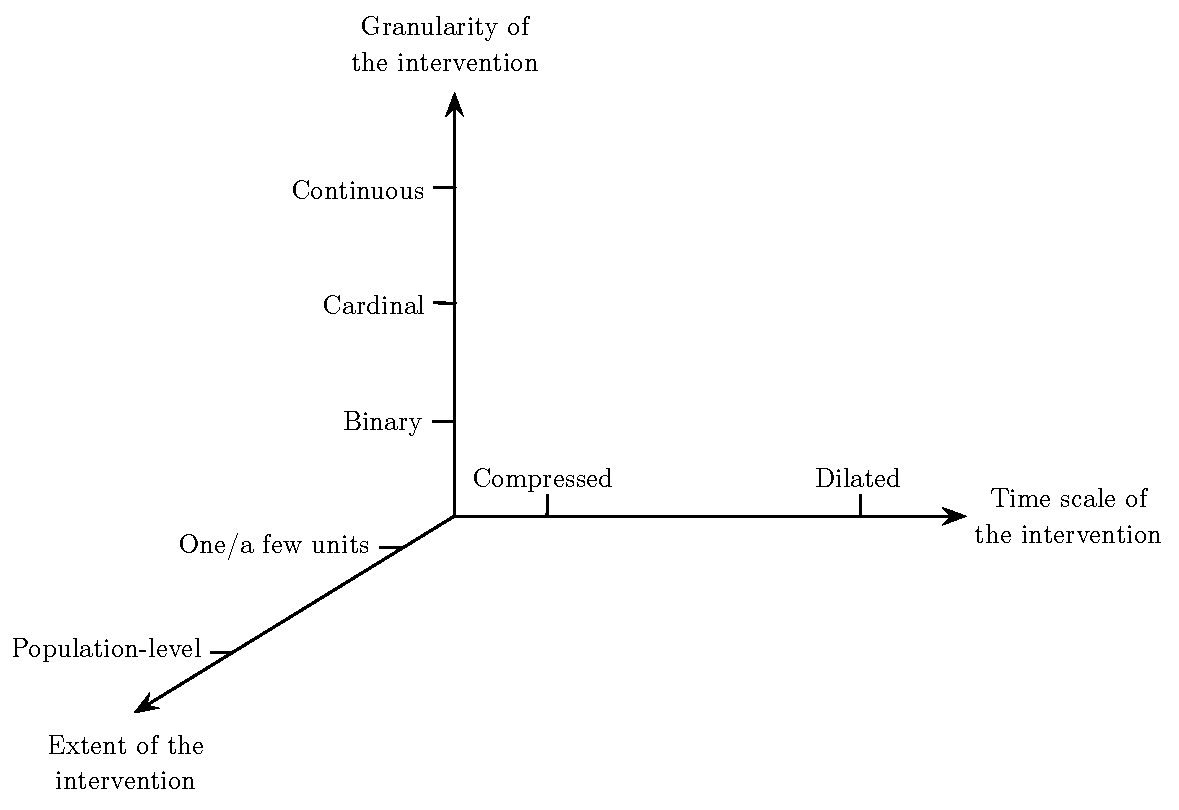
\includegraphics[width=1\textwidth]{exhibits/typology.pdf}
    \end{center}
    \caption{A typology of exogenous shocks.}
    \label{fig:typology}
\end{figure}


\section{Harnessing exogenous shocks: opportunities and challenges}
\label{sec:how_exogenous_shocks_differ}

.



\begin{figure}[!htbp]
  
\includegraphics[width=1\textwidth]{exhibits/place_holder.pdf}
  \caption{A decision tree to harnessing exogenous shocks.}
  \label{fig:harnessing_exogeneous_shocks}
\end{figure}

\section{Coda}
\label{sec:coda}
.

\clearpage

%% --------------------------- Bibliography ---------------------------------
%\bibliographystyle{plainnat}
\section*{References}
\printbibliography[heading=none]
\end{refsection}

% -------------------------- Appendix --------------------------------------
%\begin{refsection}[references/sample.bib]
%
%\section{Appendix A --- Sample of studies}
%\label{sec:sampling}
%
%\setcounter{table}{0}
%\renewcommand{\thetable}{A\arabic{table}}
%\renewcommand{\thefigure}{A\arabic{figure}}
%
%!! Describe literature search !!
%
%\subsection{References}
%
%\printbibliography[heading=none]
%
%\end{refsection}

% ----------------------------- Closing ------------------------------------
\end{document}